\chapter{Methodology and Design}
This chapter will describe the methodology used in the project. The project is mostly software based and so that will be the focus. However, there is a physical element in that of the vessel and the electrical hardware. The mechanical design and fabrication of the thruster mounts is outside the scope of this project and so it will be described only in terms of how it interfaces with the electrical hardware.\par
\section{Software Environment}
The microcontroller that was chosen for this project is a Arduino DUE. An Arduino microcontroller was chosen as there is a wide range of Arduino libraries available online, as well as several forums and code examples. Furthermore, the Arduino environment uses the C language. \par
\section{System Design}
	\subsection{Objective}
	The system needs to be designed to be deployed for long periods of time between servicing. The future addition of power regeneration such as solar or wind can be used to improve the deployable range and period of the vessel but the energy storage must be designed to handle an extended period of 'dark time', any time when the power regeneration is negligible. \par
	The vessel must be autonomous and having received a set of points before deployment, navigate between these points until retrieval. Even under non ideal circumstances the vessel should be able to correct its course and continue to navigate to the set points. \par
	This system is a proof of concept that is designed to be able sized up to a larger vessel. Therefore the prototype vessel should be able to handle any conditions that could be encountered in testing and all electronics should be sufficiently sealed so that no damage is incurred. It is not expected that the prototype vessel can handle rough and storm weather conditions.\par
	\subsection{Engineering Requirements}
	The prototype is a proof of concept that can be scaled up to a larger vessel and so a small vessel that can accommodate at least 2 people is required. This is preferred to a smaller vessel that cannot accommodate the weight of a person as the weight to power ratio of a small vessel would not be as representative and this could influence the steering capability of the vessel and therefore the control system.
	Furthermore, a working vessel is going to require a large battery bank and this is easily represented in a larger vessel. The energy source can then be scaled up by adding cells in both parallel and series to create the required power supply for the working vessel.\par
	The autonomous nature of the vessel means that the a electronic control system is required to control the vessel. Furthermore, there are several elements that are required to make up the system however, these are not integral to the autonomous nature of the system but integral to the system as a whole. All of these elements are listed in the table \ref{tab:3:elements} and will be further explained in the system description.\par
\section{System Description}
This section will give a broad overview of the system as a whole and describe the different sub-systems and their interactions. Several of these subsystems are outside the scope of the project but have been included to provide a foundation upon which the applicable detailed descriptions will build. \par
\begin{figure}
	\begin{center}
		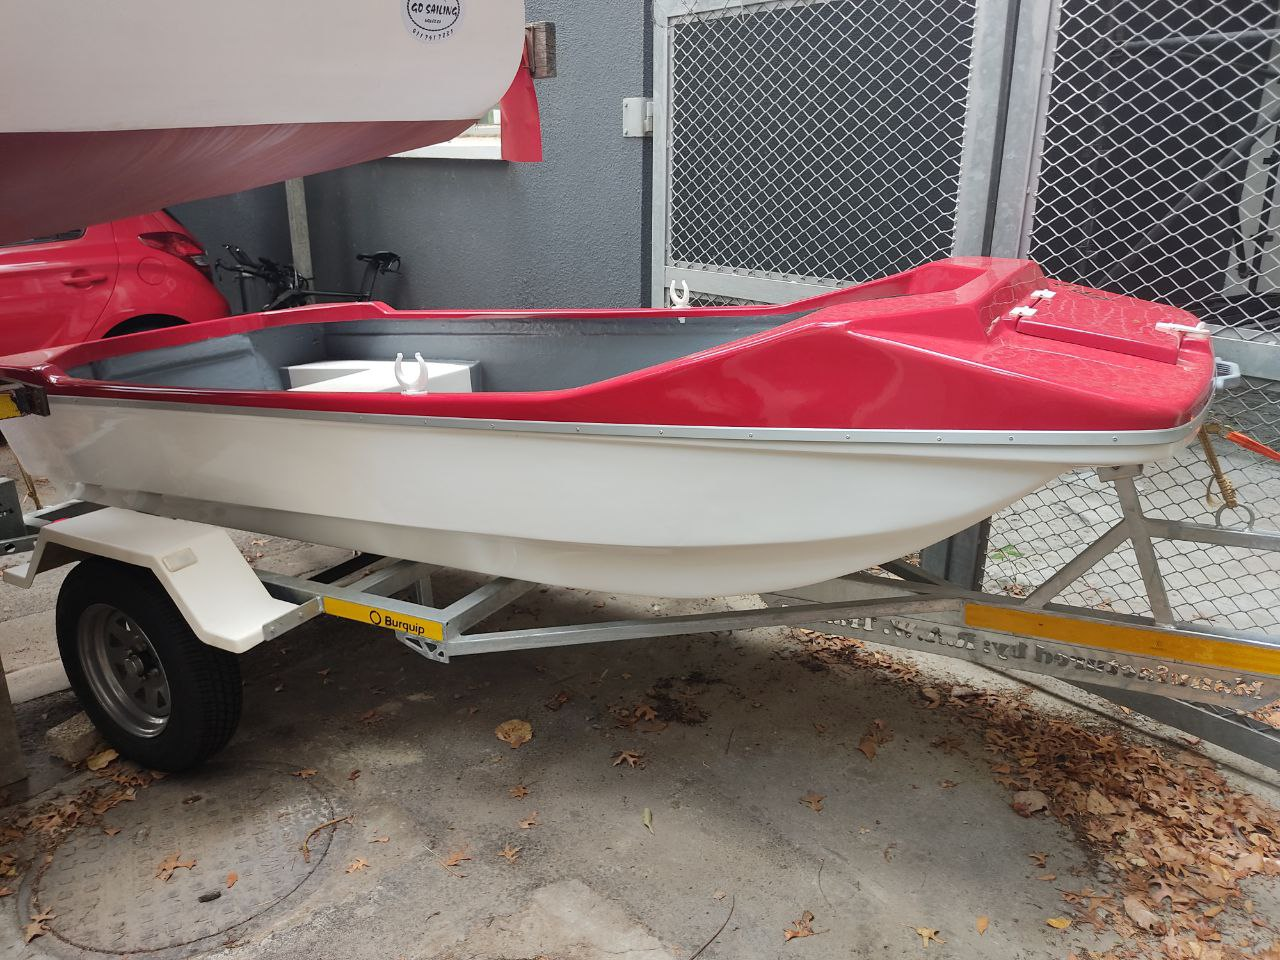
\includegraphics[width = 0.65\textwidth]{figures/spider3.jpg}
		\caption{The vessel, a spider 3.}
		\label{fig:3:spider}
	\end{center}
\end{figure}
	\subsection{Hardware}\par
		\subsubsection{Vessel}
		The vessel is outside the scope of this project as it was acquired before the start of the project. The project was designed around the use of the vessel for testing only as in actual uses the vessel would be upgraded to handle severe weather conditions and hold an array of sensory equipment. The vessel referred to in this project, pictured in figure \ref{fig:3:spider} is a Spider 3, a small single hulled fibreglass boat. The vessel measures \SI{1.3}{\meter} $\times$ \SI{3.2}{\meter} and is rated to carry 4 people and a 15hp traditional outboard motor.\par
		\subsubsection{Thrusters}
		Although the thrusters are electrical they are a complete unit together with the ESC, and all electronic interfacing was done with the ESC which then drove the thrusters. Therefore the thrusters are being considered general hardware and similarly to the boat were acquired prior to the project and are only there as a means of testing the control system. They are therefore also out of the scope of the project but are integral to the performance of the system overall.\par 
		The propulsion system consists of two electric thrusters mounted at the back of the vessel. These thrusters are each capable of producing up to \SI{18}{\kilogram} of thrust. An aliminium mount designed and manufactured by the Electrical engineering workshop allows for the thrusters to be raised during the launching and retrieval of the boat so as not to foul on the trailer. The mounts are removable and are removed for transport. Each thruster has a integrated ESC that regulates the power supplied to the electric motor and therefore the thrust provided. The ESC is detailed later in the report.
		\subsubsection{Power Supply}
		The initial design was to use a bank of 4 Lithium Iron Phosphate cells to form a \SI{12}{\volt} battery. This was also procured before the start of the project. However upon testing, it was seen that \SI{12}{\volt} was not enough voltage to provide the thrusters with enough power to move the boat at a reasonable rate. Each cell has a voltage of \SI{3.3}{\volt} and a capacity of \SI{100}{\ampere\hour}. Therefore the next course of action was to source more cells and increase the size of the battery. However, due to the high cost of these cells and a lack of suppliers this was not plausible. LiFePO cells are expensive because they are designed to have a deeper life cycle than standard lead acid cells. These cells in particular were also expensive due to their large capacity.\par 
		Finally, it was decided that in order to test the control system, the power source would be changed to a battery of two lead acid cells. The lead acid cells were each \SI{12}{\volt} and had a capacity of \SI{50}{\ampere\hour}. A lead acid battery can generally be drained to about \SI{80}{\percent} capacity without doing much damage to the cell, a LiFePO cell has a deep cycle of about \SI{40}{\percent}-\SI{50}{\percent}. Therefore these cells would be used for short tests and recharged between tests. However, for a working system it would be recommended that a large LiFePO battery bank were used. 
		\begin{figure}[!ht]
			\begin{center}
				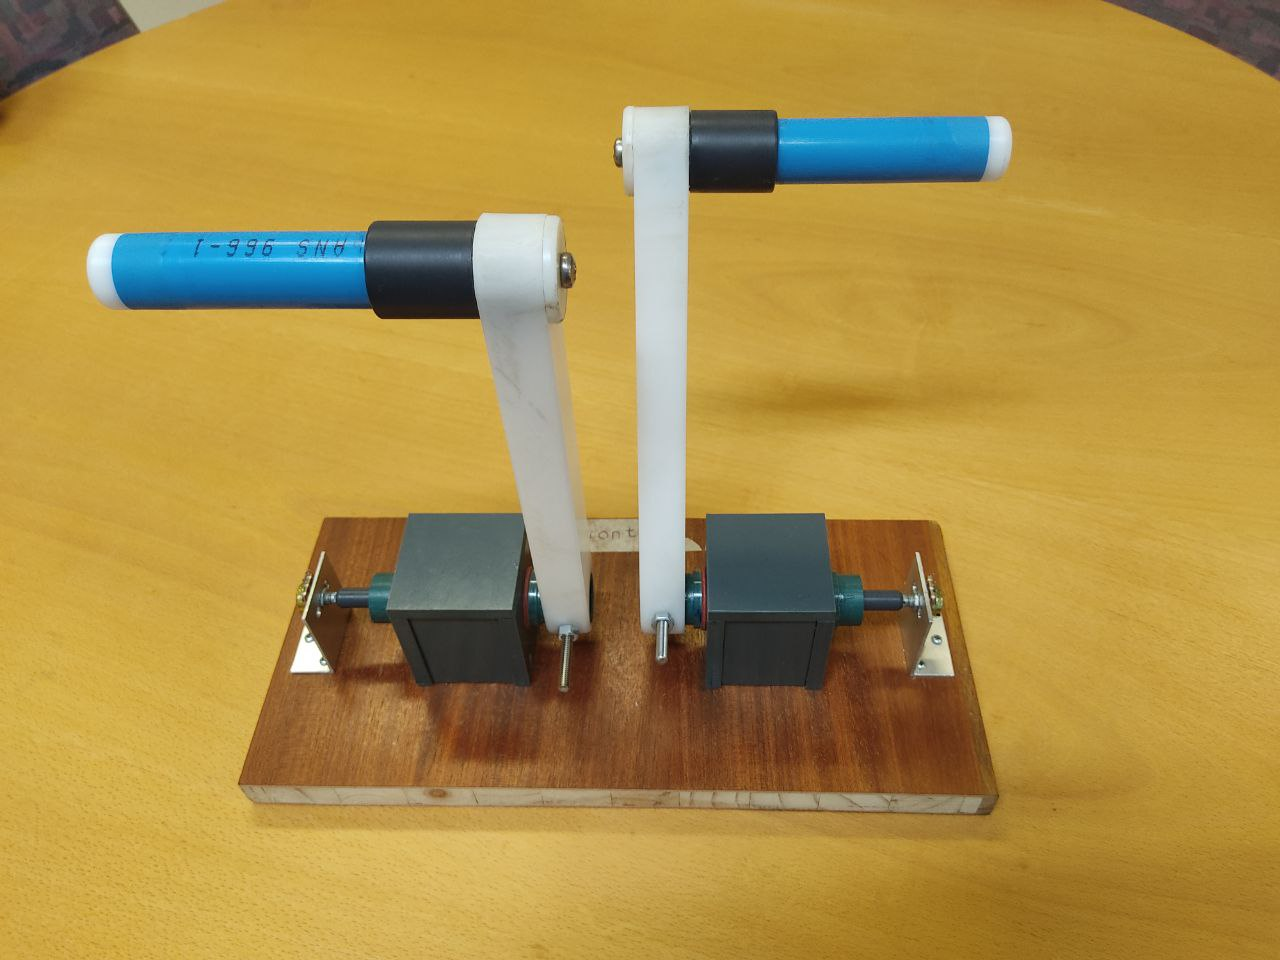
\includegraphics[width = 0.55\textwidth]{figures/throttle.jpg}
				\caption{The final throttle system with two POTs on either end.}
				\label{fig:3:throttle}
			\end{center}
		\end{figure}
		\subsubsection{Throttle}
		The initial concept was to use two throttles that can move independently from each other and %item \ref{BOM:smallThrottle} in Appendix \ref{BOM} was two electronic throttles were 
		% remove comments when BOM is in place
		purchased to be used. However, when these components arrived, they were much smaller than they had appeared and they had very small range of movement. An alternate solution was designed and consisted of two throttle arms that could each turn a shaft. This shaft was then mounted to a linear potentiometers which would provide the required analogue input from the throttle. The throttle is shown in figure \ref{fig:3:throttle}. An initial concept design was given to the electrical engineering department who then refined and manufactured the design. 
		\par
	\subsection{Electronics}\par
		\subsubsection{Arduino Due}\par
		\begin{figure}[!ht]
			\begin{center}
				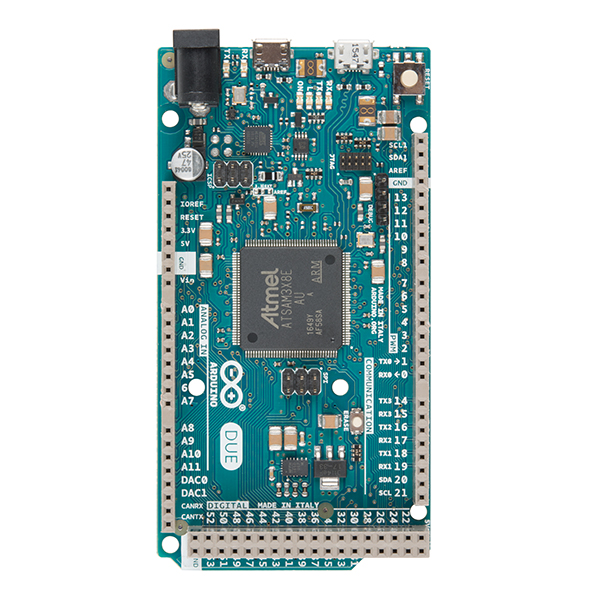
\includegraphics[width = 0.55\textwidth]{figures/DUE.jpg}
				\caption{The microcontroller used, an Arduino DUE}
				\label{fig:3:due}
			\end{center}
		\end{figure}
		The microcontroller was selected by considering the initial design and possible peripherals that would be used in the system. The minimum requirements for the microcontroller to be used with the peripherals of the GPS, SD card modules and the ESC and POTs as well as several inputs and outputs were as follows:
		\begin{enumerate}
			\item 2 PWM pins.
			\item Voltage regulators of \SI{3}{\volt} and \SI{5}{\volt}.
			\item 5 digital IO pins.
			\item 4 analogue input pins.
			\item 1 SPI connection.
			\item 1 UART connection.
			\item \SI{256}{\kilo\byte} programmable flash memory.		
		\end{enumerate}
		Based on these requirements, the Arduino Uno was considered. It is the standard Arduino board used in projects and meets most of the requirements. However, the Arduino Uno has only one UART connection and although this does meet the minimum requirements it does not allow for any possible design alterations that might need a second UART connection. Finally, the Arduino only has \SI{32}{\kilo\byte} of programmable flash memory which does not meet the requirements.\par 
		The next consideration was the Arduino DUE. This has 4 UART connections and plenty of digital IO pins and several analogue inputs. This offers a range of versatility to any design progression or alterations that might occur. Furthermore, the DUE has \SI{512}{\kilo\byte} of programmable flash memory which is double that of the minimum requirement. The one flaw with the Arduino DUE is that its IO pins operate a \SI{3.3}{\volt} as opposed to the generally standard \SI{5}{\volt}. However, this was easily overcome by implementing a logic level converter to shift the required signals to \SI{5}{\volt} while keeping the signals shape. Keeping the signals shape is particularly important for the PWM signal controlling the ESCs. The final microcontroller selected was the Arduino DUE.
		\subsubsection{SD Card Module}
		The SD card is used as an external storage device. Data can then be written to the SD card during operation and the data can be downloaded for analysis. The SD card module is a standard SD card module that is attached to the microcontroller as shown in the wiring diagram figure \ref{fig:3:wiring}. The SD card uses SPI communication and there are built in libraries that are available for use.
		\subsubsection{GPS Module}
		%Item \ref{BOM:GPS} in appendix \ref{BOM} is the GPS module used. It
		The GPS module used is a PmodGPS and it
		%remove comments when the BOM is correctly added.
		Initially a PmodGPS was used as the GPS module. However the PmodGPS has a built in antenna and there were signal strength issues. The GPS was slow at acquiring a GPS fix when the control box was closed. Therefore an alternate GPS module was sourced that has an external antenna that can be fed out of the control box and placed in a position where a strong signal can be received. Both GPS modules use UART to communicate the data to the microcontroller. The GPS modules send a string of characters along the UART connection and the microcontroller must then decode the the characters. The GPS module is used to return the current longitude, latitude, date and time, speed and heading. The UART is set-up to use a baud rate of 9600, 8 data bits, no parity and 1 stop bit.   
		has two connectors J1, which has 6 pins and J2 which has 2 pins. J1 is used to power the GPS module as well as connect to the MCU using UART communication with a baud rate of 9600, 8 data bits, no parity and 1 stop bit. 
		
		\subsubsection{ESC}
		There are two ESC, one for each thruster and are submersible and therefore they are attached to the thrusters. The ESC has two inputs, the control input and the power input. Th power input can range between DC\SI{12}{\volt} and DC\SI{50}{\volt} and a maximum constant currennt of \SI{100}{\amp} and in this project the input is \SI{24}{\volt} supplied by the battery cells. The control input is a 5V signal that is used to control the speed of the thrusters. This is a PWM signal whose duty cycle determines the thrusters speed and direction. 
		
		\subsubsection{PWM Signal}
		The thrusters are each controlled by a \SI{5}{\volt} PWM signal. There is limited information on the datasheet for the ESC and the signal boundaries, full forward, full reverse and neutral positions are described in the unconventional terms of the time that the signal is high. The values are shown in table \ref{tab:3:PWM}. Initially it was thought that the ESC operated at \SI{50}{\hertz}, however there was no response from the thruster at any duty cycle.\par
		\begin{table}[!ht]
			\begin{center}
				\caption{ESC boundaries and PWM duty cycle at various frequencies.}
				\label{tab:3:PWM}
				\begin{tabular}{|l|c|c|c|c|}
					\hline
					\multirow{2}{*}{Position} & \multirow{2}{*}{Time (\SI{}{\micro\second})} & \multicolumn{3}{c|}{Duty Cycle @}\\
					%\hline 
					& & \multicolumn{1}{c}{\SI{50}{\hertz}} & \multicolumn{1}{c}{\SI{60}{\hertz}} & \multicolumn{1}{c|}{\SI{500}{\hertz}}\\
					\hline
					Full Forward & 2000 & \SI{10}{\percent} & \SI{12}{\percent} & \SI{100}{\percent}  \\
					\hline
					Neutral & 1500 & \SI{7.5}{\percent} & \SI{9}{\percent} & \SI{75}{\percent}  \\
					\hline
					Full Reverse & 1000 & \SI{5}{\percent} & \SI{6}{\percent} & \SI{50}{\percent}  \\
					\hline
				\end{tabular}
			\end{center}
		\end{table}
		\vspace{0.4cm}
		In order to be sure that the correct PWM signal was being sent through and to be able to quickly vary both the frequency and the duty cycle, a PWM signal generator IC was connected to ESC and trial and error was conducted to determine that the ESC began responding to a signal above \SI{60}{\hertz}. It was then decided to push the frequency up to the maximum of \SI{500}{\hertz} as this would offers the finest control because it has the maximum allowable duty cycle difference between the signal boundaries.\par
		\vspace{0.4cm}
		The Arduino libraries contain a function that can output a PWM wave, given the duty cycle and the pin to output on as a parameter however, the default frequency of the Arduino DUE PWM pins is \SI{1000}{\hertz}. Therefore, the frequency had to be manually changed by changing the timer settings driving the PWM signal.\par
		\vspace{0.4cm}
		The information needed to change the timer settings is available in the Arduino Datasheet. The process to configure the PWM outputs is as follows. First, the peripheral clocks for timer channels 6 and 7 were enabled. Secondly, the pins input output controller on peripheral A needed to be disabled and the pins switch to peripheral type B. Then came the configuration of the timer itself. The channel mode was set to waveform mode using clock 1 with the counter being incremented on the rising edge. Furthermore, the waveform was set to UP mode (signal being set high) being triggered when the counter reached the register C (RC) value and the signal being cleared when the counter reached the register A (RA) value. Once the timer is configured, the RA and RC values can be filled and the interrupt set to trigger when the counter reaches RC. Finally, the channel control register is set to perform a software trigger, reset the counter and start the clock. There is also a interrupt handler that needs to be added where in the status register is read. This is done because the flags in the status register are automatically reset when the status register is read, at the end of every period.\par
		\vspace{0.4cm}
		The signal is being cleared when the counter reaches RA and set high when the counter reaches RC and so RC can be equated to the period of the signal and RA to the time when the signal is high. Using this and that the clock is set to clock 1 which is the MCU clock (MCK) divided by 2, the RA and RC can be expressed in terms of MCK, frequency and duty cycle as shown in equations \ref{eq:3:RC} and \ref{eq:3:RA}. RC is kept constant throughout while RA is changed to change the duty cycle of the PWM signal sent to the ESC and therefore control the ESC and thruster.
		\begin{equation}
			RC = \frac{\frac{MCK}{2}}{Frequency}
			\label{eq:3:RC}
		\end{equation}
		\begin{equation}
			RA = RC \times Duty Cycle
			\label{eq:3:RA}
		\end{equation}
		\subsubsection{POT}
		The POT has three pins as shown in figure \ref{fig:3:POTdraw}, high voltage, ground and the output. The high voltage and ground are connected to the connections on either side and the output is connected to the middle. The output is therefore a voltage in the range of $V_{CC}$ to GND. The Arduino DUE pins are \SI{3}{\volt} tolerant and so the $V_{CC}$ is driven by \SI{3}{\volt} signal. \par
		\vspace{0.4cm}
		\begin{figure}[ht]
			\begin{center}
				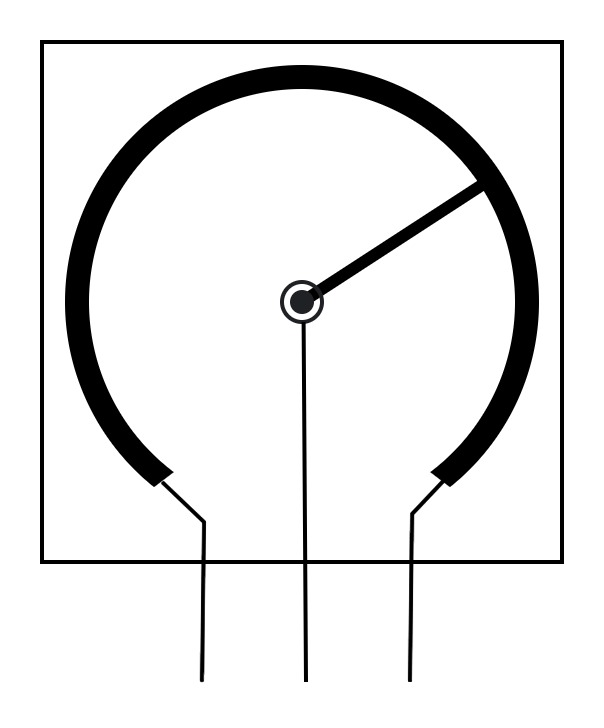
\includegraphics[width = 0.3\textwidth]{figures/POT.jpg}
				\caption{Fundamental illustration of a linear potentiometer}
				\label{fig:3:POTdraw}
			\end{center}
		\end{figure}
		The output of the POT is connected to analogue pins on the MCU and so the function, \textit{analogRead()} can be used to convert the analogue voltage into digital value using the built in ADC. The ADC has a 10 bit resolution and so the digital value is an integer in the range 0 to 1024 and the smallest discernible voltage change is \SI{3}{\milli\volt}. However, the design of the throttle does not use the full \SI{300}{\degree} range and so the physical limits needed to be measured to calibrate the throttles. The measured limits and centre points for the two throttles are shown in table \ref{tab:3:POT}. The neutral position is described by two values so that there is a neutral range that could easily be achieved by the users input. \par
		%\vspace{0.4cm}
		\begin{table}[ht]
			\begin{center}
				\caption{Measured physical limits and neutral range of the throttle POTs}
				\label{tab:3:POT}
				\begin{tabular}{|l|c|c|}
					\hline		
					\textbf{Throttle Position} & \textbf{Left POT} & \textbf{Right POT} \\
					\hline
					Full Forward & 677 & 700\\
					\hline
					\multirow{2}{*}{Neutral} &530 &540 \\
					&490 &500  \\
					\hline
					Full Reverse & 321 & 340 \\
					\hline
				\end{tabular}
			\end{center}
		\end{table}
		Using table \ref{tab:3:PWM} and \ref{tab:3:POT} a relationship can be created to determine the RA value for a given throttle position. Because the forward operation is in the duty cycle range \SI{75}{\percent} to \SI{100}{\percent}, the analogue input from the POT needs to be linearly mapped to represent an equivalent duty cycle in this range. Equation \ref{eq:3:dutyF} shows how this is done for the forwards operation. The same logic can be used to determine the duty cycle for reverse as equation \ref{eq:3:dutyR} shows. However, neutral is a set value that is written to RA whenever the throttle is within the neutral range.
		\begin{equation}
			Duty Cycle_{Forward} = 100 - (100-75)(\frac{POT_{MAX} - POT_{Input}}{POT_{MAX} - POT_{Neutral}})
			\label{eq:3:dutyF}
		\end{equation}
		\begin{equation}
			Duty Cycle_{Reverse} = 75 - (75-50)(\frac{POT_{Neutral} - POT_{Input}}{POT_{Neutral} - POT_{MIN}})
			\label{eq:3:dutyR}
		\end{equation}
	\subsection{Software}
	\subsubsection{GPS}
	 The GPS module transmits a series of 5 sentences containing various information. Each sentence begins with a '\$GP' and then the specific message ID. The data is then sent through comma separated and finally ends with a checksum and the end of line characters <CR><LF>. For this project the 'RMC' sentence is the only sentence of interest as it contains all the necessary information, longitude, latitude, speed over ground in knots and course over ground in degrees. An example of the 'RMC' sentence is shown below.\par
	\vspace{0.2cm}
	\par
	\begin{center}
		\begin{tabular}{c}
			\small{\$GPRMC,064951.000,A,2307.1256,N,12016.4438,E,0.03,165.48,260406,3.05,W,A*55<CR><LF>}\\
		\end{tabular}
	\end{center}
	\vspace{0.4cm}
	The entire sentence is read by the MCU before it starts to pick out the specific data out of the string using the commas and full stops as the guide to what array position is what data. Each piece of data is then added to an instance of a GPS structure that can then be easily parsed to the navigation algorithm and easily analysed. The variables within the GPS structure are shown in table \ref{tab:3:GPSstruct}.
	\begin{table}[!hb]
		\begin{center}
			\caption{Variables and their types within the GPS structure.}
			\label{tab:3:GPSstruct}
			\begin{tabular}{|l|l|l|}
				\hline
				\textbf{Name} & \textbf{Type} & \textbf{Description} \\
				\hline
				UTC & int & Coordinated Universal Time in the format (hhmmss). \\
				\hline
				lat & int & The whole number portion of the latitude. \\
				\hline
				latDecimal & int & The decimal portion of the latitude. \\
				\hline
				n\_s & char & A character indicating North or South. \\
				\hline
				longi & int & The whole number portion of the longitude. \\
				\hline 
				longiDecimal & int & The decimal portion of the longitude. \\
				\hline 
				e\_w & char & A character indication East or West. \\
				\hline
				knots & float & The speed over ground in knots. \\
				\hline
				course & float & The course over ground in degrees. \\
				\hline
				date & int & The date in the format (ddmmyy). \\
				\hline
			\end{tabular}
		\end{center}
	\end{table}

	\subsection{Control System}
	The control system is the intended scope of the project and consists of a manual and automated control. For manual control, there is a two lever throttle system that is used to control the thrusters. In automated control, the control system uses a GPS and digital compass to navigate to prescribed points. At the centre of this control system is the PCB motherboard containing the MCU, GPS and connections to both the throttle and the thrusters. 
\section{Control System}
The control logic of the control system is all implemented through the software on the Arduino MCU. This section will go into detail on logic and how that logic is carried out in software as well as the electronics that are used. 
%The source code that will be discussed can be seen in Appendix \ref{Code}
